\documentclass[12pt,a4paper]{article}
\usepackage{kotex}
\usepackage{amssymb}
\usepackage{graphicx}
\usepackage{hyperref}
\usepackage{indentfirst}
\usepackage{subcaption}
\usepackage{multirow}
\usepackage{flafter}
\usepackage{tikz}
\usepackage{wrapfig}
\usepackage{spreadtab}
\usetikzlibrary{arrows.meta, intersections, decorations.markings,
    positioning, backgrounds, through, calc, angles, quotes}
\setlength{\parskip}{2mm}
\usepackage{amsmath}
\usepackage[top=3cm, bottom=2.54cm, left=2.54cm, right=2.54cm]{geometry}
\usepackage[yyyymmdd]{datetime}
\renewcommand{\dateseparator}{-}
\usepackage{array}
\hbadness=99999
\newcolumntype{L}[1]{>{\raggedright\let\newline\\\arraybackslash\hspace{0pt}}m{#1}}
\newcolumntype{C}[1]{>{\centering\let\newline\\\arraybackslash\hspace{0pt}}m{#1}}
\newcolumntype{R}[1]{>{\raggedleft\let\newline\\\arraybackslash\hspace{0pt}}m{#1}}

\begin{document}
\begin{titlepage}
    \centering
    \begin{tabular}{|C{15cm}|}
        \hline
        \rule{0in}{6ex}
        {\huge 물리학 및 실험 1\par} \\ 
        {\large 로터리 모션 센서를 활용한 관성모멘트 측정\par} \\
        \hline
    \end{tabular} \\
    \vspace{5cm}
    
\includegraphics[height=7.36cm]{logo.png}\par
    \vspace{3cm}
    \begin{tabular}{|l|l|l|l|l|l|}
        \hline
        과목 & \multicolumn{5}{l|}{물리학및실험1} \\
        \hline
        담당교수 & \multicolumn{2}{l|}{전계진} & 담당조교 & \multicolumn{2}{l|}{} \\
        \hline
        조 및 조원 & \multicolumn{5}{l|}{2조, 김민수 김민규 김민서 김백준 김연주} \\
        \hline
        제출일 & \multicolumn{5}{l|}{\today} \\
        \hline
        작성자 & 김민수 & 학번 & 20518009 & 학과 & 정보보호 \\
        \hline
    \end{tabular}
\end{titlepage}
\section{서론}
\begin{itemize}
    \item 크기와 모양을 갖는 실제 물체는 힘을 가하면 회전운동을 한다.
    \item 직선운동 하는 물체의 질량이 관성의 역할을 하듯이 회전운동하는 물체의
        관성의 역할을 하는 것이 관성 모멘트이다.
    \item 강체의 회전 관성은 물체의 질량 뿐 아니라 질량이 회전축에 대해 어떻게
        분포되어 있느냐에 따라 달라진다.
    \item 여러 가지 형태의 강체들의 관성모멘트를 측정하여 관성모멘트 개념과 정의를
        이해한다.
\end{itemize}
\section{실험목적}
강체는 기하학적인 형태에 따라 관성모멘트가 다르다. 여러가지 형태의 강체들의
관성모멘트를 측정하여 관성모멘트의 개념과 정의를 이해한다.
\section{실험원리}
\subsection{관성 모멘트}
강체를 작은 입자들의 집합으로 생각하고, 이 강체가 고정된 z축을 중심으로 각속력
$\omega$로 회전한다고 가정하자. 질량을 $m_i$인 입자가 회전축으로부터 $r_i$ 떨어진
점에서 접선 속력 $v_i$로 운동하는 경우 이 입자의 운동에너지는
$$K_i=\frac{1}{2}m_iv_i^2$$
전체 운동 에너지는
$$K_R=\sum_iK_i=\sum_i\frac{1}{2}m_iv_i^2=\frac{1}{2}\sum_im_ir_i^2\omega^2$$
$$K_R=\frac{1}{2}\left(\sum_im_ir_i^2\right)\omega^2=\frac{1}{2}I\omega^2$$
(단, $\omega$=각속력, $v_i=r_i\omega$, $I\equiv\sum m_ir_i^2$=관성모멘트)
$$\textrm{회전 운동 에너지}=K_R=\frac{1}{2}I\omega^2$$
$$\textrm{관성 모멘트}=I\equiv\sum_im_ir_i^2$$
\clearpage
\begin{itemize}
    \item 관성 모멘트는 물체의 각속력 변화에 저항하는 정도.
    \item 관성 모멘트는 강체의 질량뿐 아니라 회전축에 대해 질량이 어떻게 분포하는지에
        의존한다.
\end{itemize}
회전 운동 에너지는 새로운 형태의 에너지는 아니다. 강체를 이루는 입자들의 각각의
운동 에너지의 합으로부터 유도하였으므로 일반적인 운동 에너지이다. 연속 매질 물체의
관성모멘트는 적분으로 표현된다.
$$I=\lim_{\Delta m_i \to 0}\sum_ir^2\Delta m_i=\int r^2dm$$
\begin{figure}[h!]
    \centering
    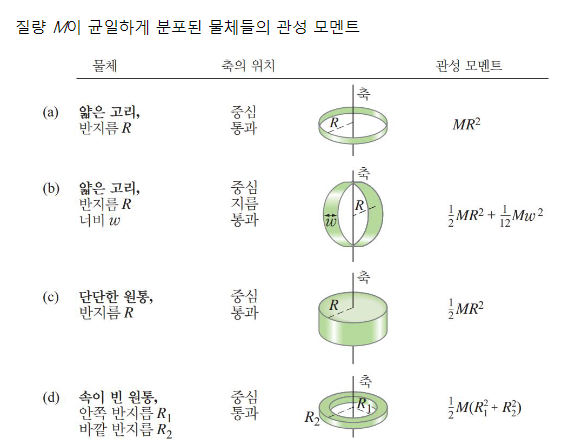
\includegraphics[width=15cm]{2024-05-26 224240.png}
\end{figure}
\begin{figure}[h!]
    \centering
    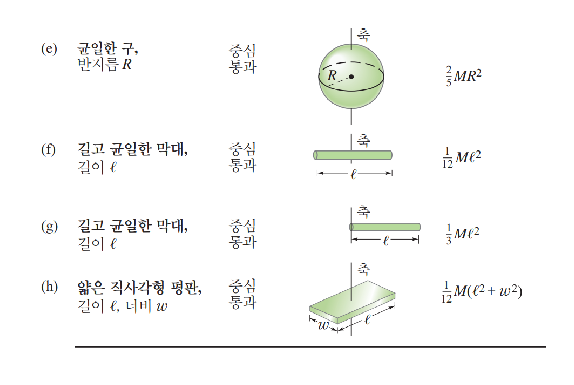
\includegraphics[width=15cm]{2024-05-26 224246.png}
\end{figure}
\clearpage
\subsection{강체의 회전운동 방정식}
물체를 회전시키기 위해서는 힘이 필요하다. 회전은 힘이 작용한 위치와 방향에 모두 
관계된다. 회전축으로 부터 힘이 작용한 선 까지의 수직거리를 지레 팔 또는 모멘트
팔이라 부른다.
\begin{figure}[h!]
    \centering
    \begin{subfigure}[]{0.4\textwidth}
        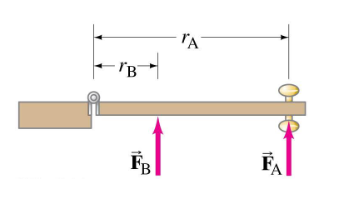
\includegraphics[width=5cm]{2024-05-26 224858.png}
    \end{subfigure}
    \begin{subfigure}[]{0.4\textwidth}
        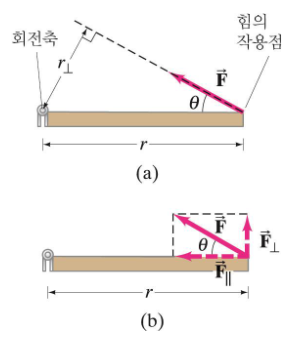
\includegraphics[width=5cm]{2024-05-26 224656.png}
    \end{subfigure}
\end{figure}
회전력(torque) 또는 돌림힘, 힘의 모멘트
$$\tau=rF\sin\theta$$
$$(\textrm{단위}: N \cdot m)$$
\begin{itemize}
    \item 강체에 작용하는 알짜 토크가 영이 아니면 각가속도의 원인이 된다.
\end{itemize}
$$\therefore\textrm{알짜토크를 받는 강체에 대해서는 회전운동에서의 뉴턴의 제2법칙}$$
$$\sum\tau_{ext}=I\alpha \textrm{ 를 사용하여야 한다.}$$
\subsection{강체의 관성모멘트 측정}
물체의 관성 모멘트를 측정 하는 방법을 생각해보자. 원반의 회전운동에서 실험적인 값을
구하기 위해 그림과 같은 실험 장치를 생각할 수 있다.
\begin{figure}[h!]
    \centering
    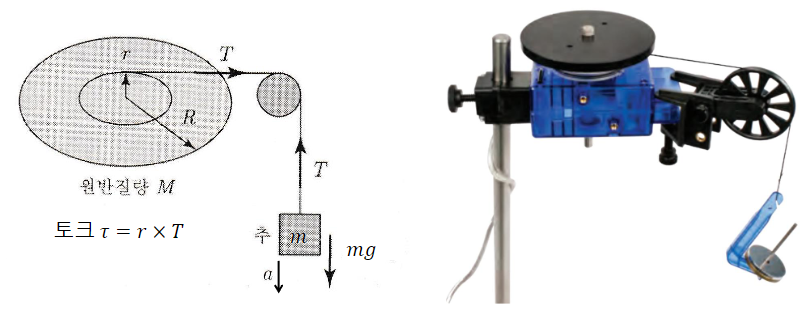
\includegraphics[width=15cm]{2024-05-26 225621.png}
\end{figure}
\clearpage
줄은 매달린 질량 $m$에 의해 당겨지고 $r$은 회전 하는 원반의 중심에 고정 부착된
도르래의 반지름이다. 작용점 $r$ 은 작용하는 힘(장력) $T$에 대해 수직이므로
회전력 $\tau$는
$$\tau=rT$$
이고 추에 대한 뉴턴 제2법칙에 따라
$$\Sigma F = ma = mg - T$$
$$\rightarrow \tau = rT = r\cdot m(g-a)$$
이다.

또한 추의 직선 가속도 $a$는 회전기구의 접선가속도 $a_{tan}$ 과 같고 각가속도
$\alpha$는
$$\alpha = \frac{a_{tan}}{r}=\frac{a}{r}$$
이다.

3단 도르래의 회전에 대한 뉴턴 제2법칙에 의하면 $\tau=I\alpha$ 이므로.
$$I=\frac{\tau}{\alpha}=\frac{r\cdot m(g-a)}{\frac{a}{r}}=mr^2(\frac{g}{a}-1)$$
와 같이 물체의 관성모멘트를 도르래를 통해 매달린 추에 의해 회전계가 회전할 때
접선 가속도를 측정함으로써 구할 수 있다
\section{실험기구 및 장치}
\begin{enumerate}
    \item 역학 실험 장치
        \begin{itemize}
            \item 관성모멘트 측정장치세트: 원반, 링, 막대
            \item 원반게이트, 3단 도르래, 도르래지지대, 중심축, 추걸이, 추세트,
                버니어켈리퍼스
            \item 스텐드, 버니어 켈리퍼, 실
        \end{itemize}
    \item 센서 실험 장치
        \begin{itemize}
            \item PC, PASCO 550 Interface, data 수집 및 분석 software(Capstone),
                회전운동 센서(Rotary motion sensor)
        \end{itemize}
\end{enumerate}
\begin{figure}[h!]
    \centering
    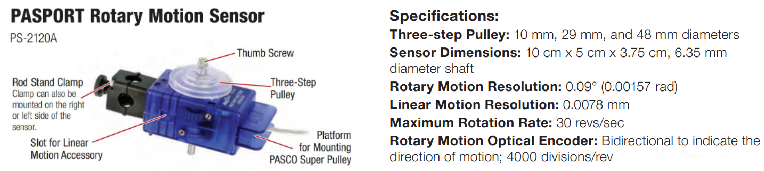
\includegraphics[width=15cm]{2024-05-26 231136.png}
\end{figure}
\section{실험방법}
\begin{enumerate}
    \item 준비
        \begin{itemize}
            \item 로터리 모션 센서 앞쪽에 도르래를 설치한다
            \item 120cm 잘라 준비한 실을 3-step pully(3단 도르래)의 중간 풀리에
                감기도록 장치한다. 이 때 3단 도르래가 헛돌지 않도록 실을 잘
                묶어준다.
            \item 실의 반대쪽에 추걸이를 매단다.
            \item 로터리 모션 센서를 550 인터페이스에 연결한다.
            \item 캡스톤 프로그램을 실행하고 속도 vs 시간 그래프를 구성한다.
            \item Sampling rate를 50 Hz로 설정한다.
            \item 3-step pully의 설정에 들어가서 medium(29mm 직경)으로 선택한다.
        \end{itemize}
    \item 강체의 관성모멘트 측정 실험
        \begin{enumerate}
            \item 회전축 자체의 강체의 관성모멘트 측정
                \begin{enumerate}
                    \item 3단 도르래의 중간 도르래의 직경을 버니어 켈리퍼스로
                        측정하여 2로 나누어서 반지름($r$)을 기록한다.(5회)
                    \item 장치를 측면과 상단에서 볼 때 일직선이 되도록 맞추고,
                        추가 스마트 풀리까지 거의 올라오도록 3단 도르래에 실을 감고
                        회전체를 잡아서 정지상태를 유지한다.
                    \item 회전체를 놓으며 RECORD버튼을 누른다. 추가 바닥에 닿기
                        전에 STOP 버튼을 누른다. 이때 추가 너무 빠르거나 느리면
                        오차가 커지므로 적당한 추의 무게를 선택한다.
                        (이때 추의 질량은 5g이 적당하다.)
                    \item 측정 종료 후, 그래프 툴바에서 fitting (추세선) 영역을
                        선택해서 1차 함수 $(mt+b)$ 로 fitting 해서 기울기
                        (가속도)를 구해서 데이터 테이블에 기록한다.
                    \item 위 과정을 5번 되풀이 한다.
                    \item 가속도 평균값을 이용하여 $I = mr^2(\frac{g}{a}-1)$식을
                        이용하여 $I_{\textrm{축}}$ 을 계산한다
                \end{enumerate}
            \item 원반의 관성모멘트 측정
                \begin{enumerate}
                    \item 측정할 원반의 반지름$(R)$과 질량$(M)$을 재어 기록하고,
                        사각 홈에 잘 맞추어 끼운 후 나사로 고정한다.
                    \item 원반이 수평이 되게 한다.
                    \item 추가 스마트 풀리까지 거의 올라오도록 3단 도르래에 실을
                        감고 회전체를 잡아서 정지상태를 유지한다.
                    \item 회전체를 놓으며 RECORD버튼을 누른다. 추가 바닥에 닿기
                        전에 STOP 버튼을 누른다. 이때 추가 너무 빠르거나 느리면
                        오차가 커지므로 적당한 추의 무게를 선택한다.
                        (이때 추의 질량은 35g이 적당하다.)
                    \item 측정 종료 후, 그래프 툴바에서 fitting (추세선) 영역을
                        선택해서 1차 함수 $(mt+b)$ 로 fitting 해서 기울기(가속도)
                        를 구해서 데이터 테이블에 기록한다.
                    \item 위 과정을 5번 반복한다.
                    \item 가속도 평균값을 $I = mr^2(\frac{g}{a}-1)$식을 이용하여
                        회전계의 관성모멘트를 측정한 다음, 축에의한 값
                        $I_{\textrm{축}}$을 빼주면 원반의 관성모멘트
                        $I_{\textrm{원반}}$이 된다.
                    \item 실험값을 구하고 이론치와 비교한다.
                \end{enumerate}
            \item 링의 관성모멘트 측정
                \begin{enumerate}
                    \item 측정할 링의 내부반경과 외부반경과 질량을 재어 기록하고
                        (5회), 원판위에 링을 올려놓는다.
                    \item 원반이 수평이 되게 한다.
                    \item 추가 스마트 풀리까지 거의 올라오도록 3단 도르래에 실을
                        감고 회전체를 잡아서 정지상태를 유지한다.
                    \item 회전체를 놓으며 RECORD버튼을 누른다. 추가 바닥에 닿기
                        전에 STOP 버튼을 누른다. 이때 추가 너무 빠르거나 느리면
                        오차가 커지므로 적당한 추의 무게를 선택한다.
                        (이때 추의 질량은 35g이 적당하다.)
                    \item 측정 종료 후, 그래프 툴바에서 fitting (추세선) 영역을
                        선택해서 1차 함수 $(mt+b)$ 로 fitting 해서 기울기(가속도)
                        를 구해서 데이터 테이블에 기록한다.
                    \item 위 과정을 5번 반복한다.
                    \item 가속도 평균값을 $I = mr^2(\frac{g}{a}-1)$식을 이용하여
                        회전계의 관성모멘트를 측정한 다음, 축에의한 값
                        $I_{\textrm{축+원반}}$을 빼 주면 링의 관성모멘트
                        $I_{\textrm{링}}$이 된다.
                    \item 평균치를 구하고 이론치와 비교한다.
                \end{enumerate}
        \end{enumerate}
\end{enumerate}
\section{실험 결과}
\begin{enumerate}
    \item 축의 관성모멘트
        \begin{enumerate}
            \item 3단 도르래의 중간 반경(2단) $r$측정(직경의 반) \\
                \\
                \begin{tabular}{|c|c|c|c|c|c|c|}
                    \hline
                    &1&2&3&4&5&평균 \\
                    \hline
                    r&0.0143&0.0144&0.0144&0.0147&0.0143&0.0144 \\
                    \hline
                \end{tabular}
            \item 추+추걸이$(m)=0.0050[kg]$
            \item 측정한 가속도 $a[m/s^2]$ \\
                \\
                \begin{tabular}{|c|c|c|c|c|c|c|}
                    \hline
                    &1&2&3&4&5&평균 \\
                    \hline
                    $a$&2.15&2.13&2.16&2.15&2.12&2.142 \\
                    \hline
                \end{tabular}
            \item 실험한 $I_{\textrm{축}}=mr^2(\frac{g}{a}-1)=
            3.70673\times10^{-6}[kg\cdot m^2]$
        \end{enumerate}
        \clearpage
    \item 원반의 관성모멘트
        \begin{enumerate}
            \item 3단 도르래의 중간 반지름 측정값$(r)=0.0144m$
            \item 원반질량$(M)=0.120kg$
            \item 원반 반경$(R)$ \\
                \\
                \begin{tabular}{|c|c|c|c|c|c|c|}
                    \hline
                    &1&2&3&4&5&평균$(m)$ \\
                    \hline
                    원반 반경$(R)$&0.0476&0.0477&0.0477&0.0476&0.0476&0.0476 \\
                    \hline
                \end{tabular}
            \item 추+추걸이$(m)=0.035[kg]$
            \item 측정한 가속도 $a[m/s^2]$ \\
                \\
                \begin{tabular}{|c|c|c|c|c|c|c|}
                    \hline
                    &1&2&3&4&5&평균 \\
                    \hline
                    $a$&0.477&0.477&0.473&0.473&0.473&0.4746 \\
                    \hline
                \end{tabular}
            \item 실험한 $I_{\textrm{원반+축}}=
                mr^2(\frac{g}{a}-1)=1.42604\times10^{-4}[kg\cdot m^2]$
            \item $I_{\textrm{원반}}=I_{\textrm{원반+축}}-I_{\textrm{축}}=
                1.388976\times10^{-4}[kg\cdot m^2]$
            \item 이론적 관성 모멘트 $I_{\textrm{원반}}=\frac{1}{2}MR^2=
                1.35946\times10^{-4}[kg\cdot m^2]$
            \item 상대 오차$=2.17\%$
        \end{enumerate}
    \item 링의 관성모멘트
        \begin{enumerate}
            \item 3단 도르래의 중간 반지름 측정값$(r)=0.0144m$
            \item 링의 질량$(M)=0.4705kg$
            \item 링의 반경$(m)$ \\
                \\
                \begin{tabular}{|c|c|c|c|c|c|c|}
                    \hline
                    &1&2&3&4&5&평균$(m)$ \\
                    \hline
                    링 내부 반경$(R_1)$&0.0266&0.0267&0.0267&0.0268&0.0268&
                        0.02672 \\
                    \hline
                    링 외부 반경$(R_2)$&0.0381&0.0383&0.0382&0.0383&0.0383&
                        0.03824 \\
                    \hline
                \end{tabular}
            \item 추+추걸이$(m)=0.035[kg]$
            \item 측정한 가속도 $a[m/s^2]$ \\
                \\
                \begin{tabular}{|c|c|c|c|c|c|c|}
                    \hline
                    &1&2&3&4&5&평균 \\
                    \hline
                    $a$&0.166&0.166&0.166&0.167&0.167&0.1664 \\
                    \hline
                \end{tabular}
            \item 실험한 $I_{\textrm{링+원반+축}}=
                mr^2(\frac{g}{a}-1)=4.20173\times10^{-4}[kg\cdot m^2]$
            \item $I_{\textrm{링}}=I_{\textrm{링+원반+축}}-I_{\textrm{원반+축}}=
                4.164664\times10^{-4}[kg\cdot m^2]$
            \item 이론적 관성 모멘트 $I_{\textrm{링}}=\frac{1}{2}M(R_1^2+R_2^2)=
                5.11964\times10^{-4}[kg\cdot m^2]$
            \item 상대 오차$=0.187\%$
        \end{enumerate}
\end{enumerate}
\clearpage
\section{고찰}
\subsection{회전운동의 관성을 나타내는 관성모멘트와 병진운동의 관성을 나타내는 질량의
    유사점과 차이점을 비교해 보세요.}
    관성모멘트와 병진운동의 질량은 둘 다 어떤 벡터값에 저항하는 정도로, 둘 다 클수록
    잘 안 멈추려고 하고 잘 움직이지 않으려고 하는 관성을 크게 가진다.
    그러나 관성 모멘트와 질량의 다른 점은 설사 질량이 같은 물체가 두개 있더라도
    물체의 질량 분포, 모양에 따라 관성 모멘트는 달라질 수 있다는 것이다.
    반면, 질량은 물체의 모양이나 질량 분포가 바뀐다고 해서 변하지 않는다.
\subsection{만일 실험에서 3단 도르래의 가장 큰 직경의 도르래를 사용하여 실험을
    한다면 측정하는 가속도는 어떻게 될 것으로 예상되는지 논하여 보세요.
    (시료의 관성모멘트는 도르래의 반경에 따라 변하지 않는다)}
    큰 직경의 도르래로 실험한다면 $I$의 값이 전체적으로 크게 나올 것 같은데, 왜냐하면
    $$I=mr^2(\frac{g}{a}-1)$$
    의 식을 이용하여 $I$의 값을 구했기에, 직경 $r$이 커지면 $I$는 $r$의 제곱에
    비례하는 관계를 갖기 때문이다.
\subsection{오차원인}
오차는 전체적으로 작게 나왔기 때문에 딱히 오차가 있었던 것 같지 않다.
있는 오차마저도 2.17\%, 0.187\%와 같이 매우 작기 때문에, 감았던 3단 도르래를 놓는
과정에서의 손의 미세한 힘, 센서의 미세한 오차, 센서의 유효자릿수와 같은 요소가 영향을
미친 것 같다, 이외에는 화성시 와우리의 중력 가속도가 정확히 $9.8m/s^2$가 되지
못했거나. 3단 도르래 센서의 미세한 마찰 등이 영향을 미친 것 같다.
\subsection{실험을 통해 배우게 된 것}
\begin{itemize}
    \item 회전운동에서 관성은 관성 모멘트로 표현된다.
    \item 관성 모멘트는 질량의 분포나 물체의 모양에 영향을 받는다.
\end{itemize}
\subsection{실험원리의 실생활에서의 예}
\begin{itemize}
    \item 엔진의 플라이휠은 보통 가운데가 빈 형상으로 제작한다.
    \item 핸드 그라인더는 스포크가 달린 가운데가 빈 형상으로 제작하지 않는다.
    \item etc..
\end{itemize}
\end{document}